\documentclass[29pt,a4paper]{moderncv}

% moderncv themes
%\moderncvtheme[blue]{casual}                 % optional argument are 'blue' (default), 'orange', 'red', 'green', 'grey' and 'roman' (for roman fonts, instead of sans serif fonts)
\moderncvtheme[green]{banking}                % idem

\usepackage[T1]{fontenc}
% character encoding
\usepackage[utf8x]{inputenc}               	% replace by the encoding you are using
\usepackage[italian]{babel}
\usepackage{color}

% adjust the page margins
\usepackage[scale=0.8]{geometry}
\recomputelengths                          	% required when changes are made to page layout lengths

\fancyfoot{} % clear all footer fields
\fancyfoot[L,RO]{\thepage}           		% page number in "outer" position of footer line
\fancyfoot[R,LO]{\footnotesize} 			% other info in 

\begin{document}
\section{\textbf{Change History:}}
\begin{tabbing}
\\\textbf{Date:} ~~~~~~~~~~~~~~~~~\= \textbf{Version Update:}~~~~~~~\= \textbf{Member:}~~~~~~~~~~~~~~~~\= \textbf{Description:}\\
2013/06/28\> 1.0 \>fractals \> Document created.\\
2013/06/28 \> 1.1 \> fractals \>Purpose added\\
2013/06/28 \> 1.2 \> fractals \>Document Conventions added\\
2013/06/28 \> 1.3 \> fractals \>Project Scope added\\
2013/06/28 \> 1.4 \> fractals \>References added\\
2013/06/28 \> 1.5 \> fractals \>System Description added \\
2013/06/28 \> 1.6 \> fractals \>Overall Architecture added\\
2013/06/28 \> 1.7 \> fractals \>Architectural Pattern added\\	
2013/06/28 \> 1.8 \> fractals \>Architectural Strategies/Tactics added\\
2013/06/28 \> 1.9 \>fractals \> Reliability added\\
2013/06/28 \> 2.0 \>fractals \> Scalability added\\
2013/06/28 \> 2.1 \>fractals \> Modifiability added\\
2013/06/28 \> 2.2 \>fractals \> Security added\\
2013/06/28 \> 2.3 \> fractals \>Performance added\\
2013/06/28 \> 2.4 \> fractals \>Usability added\\
2013/06/28 \> 2.5 \> fractals \>Integrability added\\
2013/06/28 \> 2.6 \> fractals \>Maintainability/Flexibility added\\
2013/06/28 \> 2.7 \> fractals \>Constraints added\\
2013/06/28 \> 2.8 \> fractals \>Reference Architecture added\\
2013/06/28 \> 2.9 \> fractals \>Technology and Framework Selection added\\
2013/06/28 \> 3.0 \> fractals \>Build Tools added\\
2013/06/28 \> 3.1 \> fractals \>Details of the Subsystem added\\
2013/06/28 \> 3.2 \>fractals \> Scenarios added\\
2013/06/28 \> 3.3 \>fractals \> Logical View added\\
2013/06/28 \> 3.4 \> fractals \>Development View added\\
2013/06/28 \> 3.5 \> fractals \>Physical View added\\
2013/06/28 \> 3.6 \> fractals \>Policies added\\
2013/06/28 \> 3.7 \> fractals \>Open Issues added\\
2013/06/28 \> 3.8 \> fractals \>Glossary added\\
2013/06/30 \> 3.9 \> fractals \>Purpose updated\\
2013/06/30 \> 4.0 \>fractals \> Document Conventions updated\\
2013/06/30 \> 4.1 \> fractals \>Project Scope updated\\
2013/06/30 \> 4.2 \> fractals \>References updated\\
2013/06/30 \> 4.3 \> fractals \>System Description updated\\
2013/06/30 \> 4.4 \>fractals \> Overall Architecture updated\\
2013/06/30 \> 4.5 \> fractals \>Architectural Pattern updated\\	
2013/06/30 \> 4.6 \>fractals \> Architectural Strategies/Tactics updated\\
2013/06/30 \> 4.7 \> fractals \>Reliability updated\\
2013/06/30 \> 4.8 \> fractals \>Scalability updated\\
2013/06/30 \> 4.9 \> fractals \>Modifiability updated\\
2013/06/30 \> 5.0 \> fractals \>Security updated\\
2013/06/30 \> 5.1 \> fractals \>Performance updated\\
2013/06/30 \> 5.2 \> fractals \>Usability updated\\
2013/06/30 \>  5.3 \> fractals \>Integrability updated\\
2013/06/30 \> 5.4 \> fractals \>Maintainability/Flexibility updated\\
2013/06/30 \> 5.5 \> fractals \>Constraints updated\\
2013/06/30 \> 5.7 \> fractals \>Reference Architecture updated\\
2013/06/30 \> 5.8 \> fractals \>Technology and Framework Selection updated\\
2013/06/30 \> 5.9 \> fractals \>Build Tools updated\\
2013/06/30 \> 6.0 \> fractals \>Details of the Subsystem updated\\
2013/06/30 \> 6.1 \> fractals \>Scenarios updated\\
2013/06/30 \> 6.2 \> fractals \>Logical View updated\\
2013/06/30 \> 6.3 \> fractals \>Development View updated\\
2013/06/30 \> 6.4 \> fractals \>Physical View updated\\
2013/06/30 \> 6.5 \> fractals \>Policies updated\\
2013/06/30 \> 6.6 \> fractals \>Open Issues updated\\
2013/06/30 \> 6.7 \> fractals \>Glossary Updated\\
2013/08/22 \> 6.8 \>fractals \> Purpose updated\\
2013/08/22 \> 6.9 \> fractals \>Document Conventions updated\\
2013/08/22 \> 7.0 \> fractals \>Project Scope updated\\
2013/08/22 \> 7.1 \> fractals \>References updated\\
2013/08/22 \> 7.2 \> fractals \>System Description updated\\
2013/08/22 \> 7.3 \> fractals \>Overall Architecture updated\\ 
2013/08/22 \> 7.4 \>fractals \> Architectural Pattern updated\\	
2013/08/22 \> 7.5 \> fractals \>Architectural Strategies/Tactics updated\\
2013/08/22 \> 7.6 \> fractals \>Reliability updated\\
2013/08/22 \> 7.7 \> fractals \>Scalability updated\\
2013/08/22 \> 7.8 \> fractals \>Modifiability updated\\
2013/08/22 \> 7.9 \> fractals \>Security updated\\
2013/08/22 \> 8.0 \> fractals \>Performance updated\\
2013/08/22 \> 8.1 \> fractals \>Usability updated\\
2013/08/22 \> 8.2 \>fractals \> Integrability updated\\
2013/08/22 \> 8.3 \>fractals \> Maintainability/Flexibility updated\\
2013/08/22 \> 8.4 \>fractals \> Constraints updated\\
2013/08/22 \> 8.5 \>fractals \> Reference Architecture updated\\
2013/08/23 \> 8.6 \>fractals \> Technology and Framework Selection updated\\
2013/08/23 \> 8.7 \>fractals \> Build Tools updated\\
2013/08/23 \> 8.8 \>fractals \> Details of the Subsystem updated\\
2013/08/23 \> 8.9 \>fractals \> Scenarios Diagrams updated\\
2013/08/23 \> 9.0 \>fractals \> Logical View Diagrams updated\\
2013/08/24 \> 9.1 \>fractals \> References updated\\
2013/08/24 \> 9.2 \>fractals \> System Description updated\\
2013/08/24 \> 9.3 \>fractals \> Overall Architecture updated\\
2013/08/24 \> 9.4 \> fractals \> Reliability updated\\
2013/08/24 \> 9.5 \> fractals \>Modifiability updated\\
2013/08/24 \> 9.6 \> fractals \> Integrability updated\\
2013/08/24 \> 9.7 \> fractals \> Usability updated\\
2013/08/24 \> 9.8 \> fractals \> Maintainability/Flexibility updated\\
2013/08/24 \> 9.9 \> fractals \> Constraints updated\\
2013/08/24 \> 10.0 \> fractals \> Details of Subsystem removed\\
2013/08/24 \> 10.1 \> fractals \> Index page updated\\
2013/08/24 \> 10.2 \> fractals \> Login Use Case Added\\
2013/08/24 \> 10.3 \> fractals \> Login Use Case: Services Contract Added \\
2013/08/24 \> 10.4 \> fractals \> Login Use Case: Functional Requirements \\ \> \> \> added\\
2013/08/24 \> 10.5 \> fractals \> Login Use Case: Activity Diagram added\\
2013/08/24 \> 10.6 \> fractals \> Messaging Use Case added\\
2013/08/24 \> 10.7 \> fractals \> Messaging Use Case: Services Contract added\\
2013/08/24 \> 10.8 \> fractals \> Messaging Use Case: Functional Requirements\\ \> \> \> added\\
2013/08/24 \> 10.9 \> fractals \> Messaging Use Case: Activity Diagram added\\
2013/08/24 \> 11.0 \> fractals \> View Contact List Use Case Added\\
2013/08/24 \> 11.1 \>fractals \> View Contact List Use Case: Services Contracts\\ \> \> \> added\\
2013/08/24 \> 11.2 \> fractals \> View Contact List Use Case: Functional\\ \> \> \> Requirements Added\\
2013/08/24 \> 11.3 \> fractals \> View Contact List Use Case: Activity Diagram\\ \> \> \> added\\
2013/08/24 \> 11.4 \> fractals \> Exit Use Case added\\
2013/08/24 \> 11.5 \> fractals \> Exit Use Case: Services Contracts added\\
2013/08/24 \> 11.6 \> fractals \> Exit Use Case: Functional Requirements added\\
2013/08/24 \> 11.7 \> fractals \> Exit Use Case: Activity Diagram added\\
2013/08/24 \> 11.8 \> fractals \> Technology and Framework Selection updated\\
2013/08/24 \> 11.9 \> fractals \> Open Issues updated\\
2013/08/24 \> 12.0 \> fractals \> Glossary updated\\
2013/08/24 \> 12.1 \> fractals \> Policies updated\\
2013/08/24 \> 12.2 \> fractals \> Document Conventions updated \\
2013/08/24 \> 12.3 \> fractals \> Technology and Framework updated\\
2013/08/24 \> 12.4\> fractals \> Login Use Case. View Contact Use Case,\\ \> \> \> Messaging Use Case and \\ \> \> \> Exit Use Case updated\\
2013/08/24 \> 12.5 \> fractals \> Exit Use Case: Activity \\ \> \> \> Diagram updated\\
2013/09/10 \> 12.6 \> Michelle Peens \> Updated the document purpose.\\
2013/09/10 \> 12.7 \> Michelle Peens \> Updated overall and reference architectures\\
2013/09/10 \> 12.8 \> Michelle Peens \> Added architecture requirements\\
2013/09/14 \> 12.9 \> Janine Venter \> Project Scope updated\\
2013/09/14 \> 13.0 \> Janine Venter \> System Description updated\\
2013/09/14 \> 13.1 \> Janine Venter \> Support for Latex and Mimetex libraries \\ \> \> \> updated\\
2013/09/14 \> 13.2 \> Janine Venter \> Messaging updated\\
2013/09/14 \> 13.3 \> Janine Venter \> Overall Architecture updated\\
2013/09/14 \> 13.4 \> Janine Venter \> Index page updated\\
2013/09/14 \> 13.5 \> Janine Venter \> Should update figure for architecture reference \\ \> \> \> adding the mimetes and view of image \\ \> \> \> as components\\
2013/09/14 \> 13.6 \> Janine Venter \> Updated: Application Layer, Application \\ \> \> \> Framework, Libraries, Runtime Modules, \\ \> \> \> Back-End\\
2013/09/14 \> 13.7 \> Janine Venter \> Reliability updated\\
2013/09/14 \> 13.8 \> Janine Venter \> Scalability updated\\
2013/09/14 \> 13.9 \> Janine Venter \>Modifiability updated\\
2013/09/14 \> 14.0 \> Janine Venter \> Security updated\\
2013/09/14 \> 14.1 \> Janine Venter \> Performance updated\\
2013/09/14 \> 14.2 \> Janine Venter \> Integrability updated\\
2013/09/14 \> 14.3 \> Janine Venter \> Maintainability updated\\
2013/09/14 \> 14.4 \> Janine Venter \> Build Tools updated\\
2013/09/14 \> 14.5 \> Janine Venter \>System Diagrams: Use Cases updated\\
2013/09/14 \> 14.6 \> Stephan Botha \> Use case added for  Preview and Create \\ \> \> \> MimeTeX equation\\
2013/09/14 \> 14.7 \> Stephan Botha \> Activity diagram added for Preview and \\ \> \> \> Create MimeTeX equation\\



\end{tabbing}


\newpage
\section{\textbf{Table of Contents:}}
\begin{tabbing}
\\\textbf{Subject}: ~~~~~\= ~~~~~~~~~~~~~~~~~~~~~~~~~~~~~~~~~~~~~~~~~~~~~~~~~~~~~~~~~~~~~~~~~~~~~~~~~~~~~~~~~~~~~~~\= \textbf{Page}:
\\\newline
1. Introduction \> \> 6\\							
\> 1.1 Purpose 	\> 6\\							
\> 1.2 Document Conventions\> 6 					\\
\> 1.3 Project Scope \> 6							\\
\> 1.4 References \> 6							\\
2. System Description \> \> 7					\\
3. Overall Architecture \> \> 8				\\
\> 3.1 Architectural Pattern \> 8 				\\
\> 3.2 Architectural Strategies/Tactics \> 10 	\\
\> Reliability \> 10							\\
\> Scalability 	\> 10						\\
\> Modifiability \> 10							\\
\> Security	\> 11					\\
\> Performance \> 11						\\
\> Usability \> 11							\\
\> Integrability \> 11						\\
\> Maintainability/Flexibility \> 11		\\
\> Constraints \> 12						\\
\> 3.3 Reference Architecture \> 12			\\
\> 3.4 Technology and Framework Selection \> 13 		\\
\> 3.3 Build Tools \> 13							\\
4. System Diagrams \> \> 14\\
\> 4.1 Login Use Case \> 14\\
\> 4.1.1 Services Contract \> 14\\
\> 4.1.2. Functional Requirements \> 14\\
\> 4.1.3 Sequence Diagram \> 15\\
4.2 View Contact List Use Case \> \> 16\\
\> 4.2.1 Services Contract \> 16\\
\> 4.2.2. Functional Requirements \> 16\\
\> 4.2.3 Sequence Diagram \> 17\\
4.3 Messaging Use Case \> \> 18\\
\> 4.3.1 Services Contract \> 18\\
\> 4.3.2. Functional Requirements \> 18\\
\> 4.3.3 Sequence Diagram \> 19\\
4.4 Exit Use Case \> \> 20\\
\> 4.4.1 Services Contract \> 20\\
\> 4.4.2. Functional Requirements \> 20\\
\> 4.4.3 Sequence Diagram \> 20\\
4.5 MimeTeX Use Case \> 21\\
\> 4.5.1 Services Contract\> 21 \\
\> 4.5.2 Functional Requirements \> 21 \\
\> 4.5.3 Activity Diagram \> 22\\
5. Policies \> \> 23			\\					
6. Open Issues \> \> 23			\\				
7. Glossary \> \> 23 			\\				

\end{tabbing}
\newpage
	%\maketitle
	%\vspace{-10mm}
	%Section
	\section*{\textbf{1. Introduction}}
	\vspace{4mm}
	
		\textbf{1.1 Purpose}
			\\The purpose of this document is to provide our client with a high level overview of the architecture specification including architectural strategies or tactics and patterns that will form a basis for the development of the LaTeX Chat Application. The overall outline of these concepts and how they are implemented will provide our team with a means to achieve the given set of requirements as previously agreed upon in the Requirements and Design document. This document is also meant to describe the architecture requirements needed to achieve our final goal.\\
		\vspace{1mm}
		
		\noindent \textbf{1.2 Document Conventions}
			\begin{itemize}
				\item Document Formatting: LaTeX
				\item UML Diagrams: Diagram Designer, Visual Paradigm
			\end{itemize}
		\vspace{5mm}
		%Section
		
		\noindent \textbf{1.3 Project Scope}
			\\The aim of the project is to develop an open source android XMPP chat client which supports the embedded LaTeX base equations which are rendered as images. LaTeX based equations will be rendered on the handset to produce mathematical equations. Our system will also provide the ability to view, edit and correct equations before sending.
			\parindent 5mm The application will provide a similar functionality to yaxim. Exchange of images and mathematical expressions will be possible through our software solution. The TeXchat application will have the ability to show a preview of the entered text send the equation as LaTeX code and then render it on the receiving end on the client handset.
			
		\vspace{5mm}
		
	\noindent \textbf{1.4 References}
		\begin{itemize}
		\item Mr. Will van Heerden.
			\item MSDN Authors. Chapter 3: Architectural Patterns and Styles. 
			\\{[Online]} Available at: http://msdn.microsoft.com/en-us/library/ee658117.aspx
			\\{[Accessed 21 June 2013].}
			
			\item Android Authors, 2013. Android NDK.\\ {[Online]} Available at: http://developer.android.com/tools/sdk/ndk/index.html
				\\{[Accessed 18 August 2013].}
		\end{itemize}
		\vspace{5mm}
		
	%Section
\newpage
	\section*{\textbf{2. System Description}}
	\vspace{4mm}
		\noindent The goal of our software application is to provide a chat service that will allow users to exchange messages and also to send mathematical equations in a rendered image format.  The application is intended to provide a service to users that require the ability and support for a chat client that allows them to communicate more efficiently and effortlessly in a scientific, and mathematical context.  It will provide a more usable mobile version of a Latex chat application.\\ 
		
		\noindent\textbf{Support for LaTeX and MimeTeX Libraries}
		\\The final application will have to make use of a Latex based library for the rendering of equations as images on the mobile device. For this reason we have implemented support for the MimeTeX library, through the use of the Android NDK (Native Development Kit), which allows us to embed the native C/C++ code of the MimeTeX library, in the source code of this release. The library is compiled through Eclipse using a special makefile that sets specific compiler flags to indicate that it is in math mode and not text mode.\\
		
		
		\noindent\textbf{Messaging}
		\\Our final goal is for messaging to be possible between multiple clients, and the support for sending Latex based equations, rendered on the client side and displayed as images on the handheld device. In this release however, our server supports two initial users, and have capabilities for them to send plain text messages and display these in a easy to understand manner.  
		\parindent 5mm The ability to create, render, view and send mathematical equations have been implemented and is currently working. It is now possible to send and receive these equations in image format between the two clients.
		These messages should be stored statically on the device for later retrieval.  For this purpose a SQLite database was implemented.\\
		
		\noindent\textbf{Login}
		\\A user should be authenticated by some type of login component.  This has been implemented during the initial phases of development of this application.  The server that our application uses provides the basic functionality for this authentication component, and uses a username and password based authentication method.
		
		
	\vspace{5mm}
	
\newpage	
	%Section
	\section*{\textbf{3.Overall Architecture}}
	\vspace{4mm}
		\noindent The architectural framework chosen for the application will be based on the Model View Controller(MVC) architecture in combination with the Client-Server architecture. The Operating System on which the system will be developed is Windows using Eclipse as the development tool, with Android development capabilities and the programming languages are Java, XML and as a native java language, C and C++. The MimeTeX libraries were developed using C/C++.
		
		\parindent 5mm The MVC reference architecture will allow us to separate the view (the user interface of the Android application itself),  controller (the actual coding that will handle the LaTeX rendering and the message sending and connection of clients to the server) and the model (the database that will be found on the server given to us).
		
		\parindent 5mm The Client-Server architecture will be present when it comes to the actual connection of the clients to the server. This is where a lot of contention will be present. The Client-Server architecture will be encapsulated inside the MVC architecture.\\

		\noindent \textbf{3.1 Architectural Pattern}
			\\As mentioned previously our system will be using the MVC reference architecture, and follow a client server approach. This method will allow us to separate presentation specifics from the overall control, as well as provide the support of multiple clients. The high level architecture for our application will be the Android Application Component Architecture.  The layered high level view is depicted below, outlining the applications, application framework, libraries, runtime  and relevant back end components. The overall structure of the model is depicted below:\\
\newpage
				\noindent\begin{figure*}
				\centering
				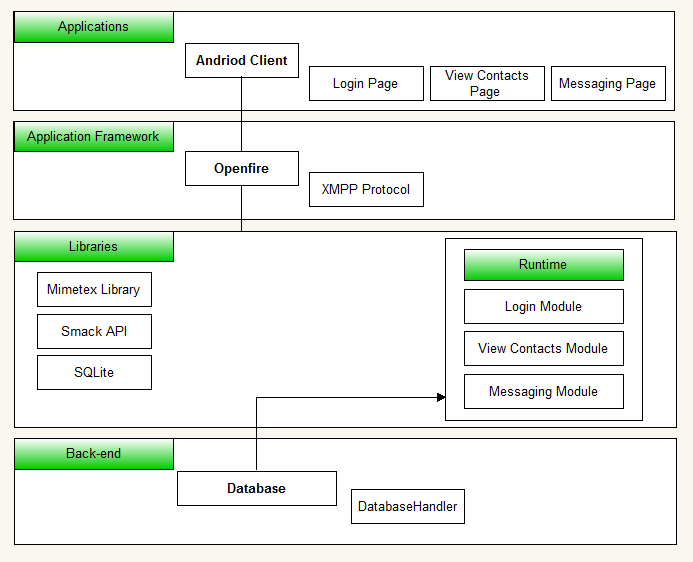
\includegraphics[width=6.0in, height=5.0in]{./overall_arch.png}
				\\\caption{[Figure 1] Overall Architecture}
				\end{figure*}\\ 
			% % % % % % % % % % % % % % % % % % % % %
			\\ \noindent\textbf{Application Layer}\\
			This layer provides the client interface to the application.\\
			
			\noindent\textbf{Application Framework}\\
			This layer outlines the server used (Openfire) and provides the connection between the clients. Moreover the protocols through which the communication is achieved is also specified.\\
			
			\noindent\textbf{Libraries}\\
			These libraries are used within the various modules of the application. (MimeTeX, SQLite, Smack)\\
			
			\noindent\textbf{Runtime mMdules}\\
			The modules that make up the application.  Each module is integrated into the application. (Login, View Contacts, Messaging, Render MimeTeX)\\
			
			\noindent\textbf{Back-End}\\
			This layer contains the functionality that the user is unaware of while using the application and includes at this point only the database for storing data relevant to a user while interacting and communication with other users. (Database).\\
			
		\vspace{5mm}
\newpage		
		\noindent \textbf{3.2 Architectural Strategies/Tactics} \\
			\\ \textbf{Reliability} 
				\\The technology and framework we will be using, such as, Openfire, will provide a very reliable server for hosting our clients. It is already implemented with multiple backup servers, and we will build our application using that. This component, provided by the server itself, is included in the current release for this iteration.
				
				We will also add a component dedicated to ensuring that messages do deliver after a client has sent it, and report an error if it failed. This will use methods such as heartbeat or ping. This will make the chat more reliable in ensuring that communication lines remain available. This component is not included in the current release of the application, and will be added during the next iteration phases of the software solution. 
				
				We will implement a backup database component to ensure that data relating to clients and messages remain reliable and available while the application is running. This component needs to ensure that a fail-over database remains available. The component has been implemented, and will be expanded on in later iterations of the application during development.
				\\
			
			\noindent\textbf{Scalability}\\
				The application at this phase of development will support only one client chat, thus it is able to support the two users that are participating in the chat. The provided server and database will allow for more than two users, but this kind of support for multiple clients will only be expected on the next release of the software. 
				
				We also need to consider the available size for the SQLite database on the client side (on the device itself), to ensure that data such as client information and chat history doesn’t grow too large for the space available. This is where a database cleanup from the client side will be made available in the next release.
				
				This may happen with previous chat histories that a user may want to retrieve or view at a later stage. Our tactic to ensure that this memory usage doesn’t grow too large will be a component to periodically delete the earliest n (some integer value greater than 0) message entries that have been in the database for long periods of time. This will remove stale data that will take up unnecessary space.  At this point of development the only database functionality included, is the retrieval of all message information ordered by date and time, thus the deletion of message will be included at a later phase of development.\\
			
			\noindent\textbf{Modifiability}\\
			The agile methodology that we are following throughout this project (RUP) will assume changes in the requirements and the design will have to be modifiable to compensate for these future changes.
			
			For instance we will need the system to eventually be able to support more than the initial amount of users (which at this point in time is two), thus supporting multiple clients participating in separate chat instances.  In this release of the application we will only be supporting the one chat instance between two users, but the system’s design at this point is relatively modifiable, and support for multiple chat instances may be easily implemented. Integrating and developing the system to support more than two clients will be realtively easy, especially if an online server such as Jabber.org is used (in this case we are using a local server and will later upgrade to an online server) If the online server is used it will also solve the scalability issue ofm supporting more than two concurrent users.
			
			Users may want other features such as changing background colours to suite their profile or their personal preference to the display of the chat client. Thus the application has to be modifiable to later include such user specific features and also extra options and features.  This component may only be expected in a later version of the design.  The current iteration phase will only display necessary information, and not provide any additional design and presentation semantics.
			\\  			
			
			\noindent\textbf{Security}\\
				One of the nice-to-have features will be that Messages sent via the chat application will be encrypted when sent and decrypted when received. This will make them secure and unobtainable by outside sources. This will also provide privacy between two users when using the application. We will provide a component or function to provide the encryption and decryption mechanics in a later phase of the development. (This has not yet been implemented)\\
			
			\noindent\textbf{Performance}\\
				Messages need to be delivered within reasonable time therefore we will add a component to avoid contention on the network between the various clients. The performance of the application will also be tested with more and more active users, exchanging messages concurrently. Analysis for this component will be done during the testing phases of our development process, and thus will not be provided in this current version of the application.
				The performance of the rendering of the MimeTeX (mathematical) equations will not be a problem because it is rendered on the device itself and not on a server. As long as the device has an operating system later than or including from Android 2.2, with the underlying hardware supported by 2.2.\\
				
			\noindent\textbf{Usability}
				\\Our final goal for this project is to develop an application that is intuitive and easy to use.  Therefore we need our design to be as simple as possible while still providing the needed or required functionality as provided by our client.  This version of the project is not as user friendly as we intend for the final product to be.  At this point it works on a basic Android device.  
				
				\\User friendliness will be analyzed once the core functionality, as requested by our client, has been included, and user testing will be done at a later stage of development.
				\begin{itemize}
					\item The application should be intuitive.
					\item It should be easy to use.
					\item The design should be simple.
					\item It should be able to work on the most basic Android device.\\
				\end{itemize}
				
			\noindent\textbf{Integrability}\\
				The application is currently being developed using Eclipse as the development tool, which has Android development capabilities.  Thus the core programming languages are Java and XML.  For our application to support the Mimetex library we have in this release started implementing components for the integration of C and C++ languages as native development languages in our application.  For this integrability requirement we have used the Android NDK (Native Development Kit).
				\\
							
			\noindent\textbf{Maintainability/Felxibility}
				\\Using a set of coding standards will allow us to reuse code and increase efficiency and reducing redundancy. This will make our source code easy to read and modify if needed by parties that aim to develop the project further.  This standard has been implemented from the initial phases of development and will remain consistent throughout the development process.
				
				The application will have a low maintainability factor regarding the server since the server that is used is an open source server, and will provide all the maintenance needed.
				
				Additional maintenance will have to be done on the client side, namely on the android application itself.  These maintenance components will include database deletion for messages that have been in the database for too long periods of time.  This database maintenance component will be implemented in later iterations and aims to increase performance on the client side. 
				The client will also get the option to delete an entire chat with another client (This will also be implemented in the next iteration.)
				
				Documentation for the application will also be provided as a hard copy.  We also intend to include a user manual document within the application itself, to provide the user of the device with additional help and needed information while using the application. This will aim to increase user satisfaction and overall usability for the application.  This component will only be implemented at a later stage of development, and thus not included in this version of the application.
				
				Unit testing will be done during the iterations of the releases and summaries of these will also be provided with the final project in the end.\\
				
			
			\noindent\textbf{Constraints}
				\\The constraints of the physical device might be an issue, designing the application in such a manner that it is still intuitive and user friendly with regard to issues such as a person being able to see the rendered image clearly even if their device has a small or limited screen display.
				
				Another issue will be whether the libraries such as the Mimetex library will be reliable enough for the application’s needs will be analysed in the next iteration of development.
		\vspace{5mm}
		
		\noindent \textbf{3.3 Reference Architecture}
			\\Our reference architecture will be the Model View Controller (MVC) architecture. It is a well known architecture that has proven to solve known web application problems, and will allow us to incorporate concepts of separating the representation of the data from a user’s ( or android client’s) interaction with it.  This way we can keep the data safe from the client aspect of our system, and only provide it with the allowed functions or methods to alter, view or retrieve the data as required by the user, via the control mechanism.\\
			
			\noindent\begin{figure*}
							\centering
							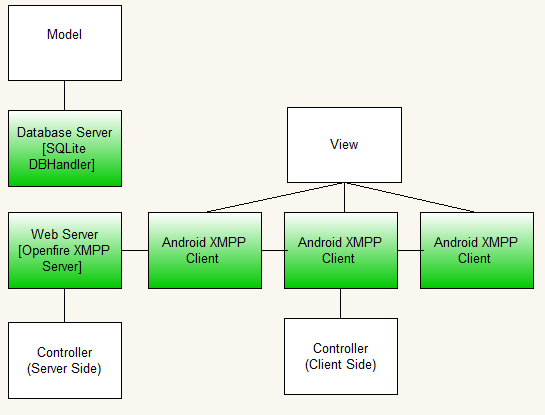
\includegraphics[width=5.5in, height=4.0in]{./OverallArchitecture.png}
							\\\caption{[Figure 2] Model-View-Controller and Client-Server Architectural Model}
							\end{figure*}
			
		\vspace{5mm}
\newpage		
		\noindent \textbf{3.4 Technology and Framework Selection}
			\begin{itemize}
				\item Android SDK, NDK
				\item Technology: Java, XML, C
				\item Frameworks: Android Application Component Architecture
			\end{itemize}
		\vspace{5mm}
		
		\noindent \textbf{3.5 Build Tools}
			\begin{itemize}
				\item We will be using Eclipse IDE and Android SDK software to build the Android Application, as well as the NDK software.
				\item We will be using the Android ADT plugin to test the application. 
				\item The application will then be distributed at a final stage on Google PlayStore and SourceForge.
				
			\end{itemize}
		\vspace{5mm}
	\vspace{5mm}	
\newpage
	\section*{\textbf{4. System Diagrams}}
	\vspace{2mm}
	 \left\textbf{4.1 Login Use Case}\\
		\\ \begin{figure*}
			\centering
			\\ 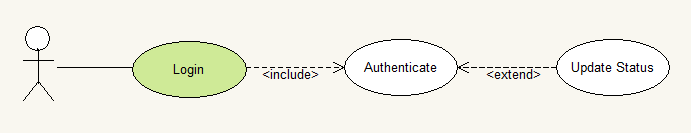
\includegraphics[width=5.8in, height=1.1in]{./loginCase.png}
			\\\caption{[Figure 2]Login Use Case}
		\end{figure*}\\
	
		\\ \noindent\textbf{4.1.1 Services Contract}\\
		To be added.\\
		
		\noindent\textbf{4.1.2 Functional Requirements}
			\begin{itemize}
				\item A secure login
				\item Log in with username, password combination.
				\item Authentication is server side.
				\item Status stored in server database.
				\item Option to remember username and passwod (stored locally on device then)\\			
			\end{itemize}
			
\newpage	
			\left\textbf{4.1.3 Sequence Diagram}\\
			\\ \begin{figure*}
				\centering
			\\	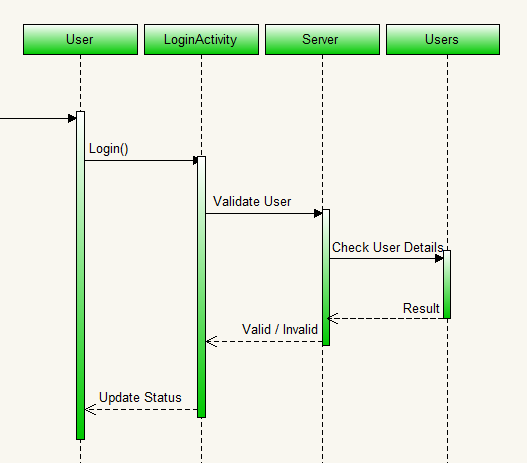
\includegraphics[width=5.5in, height=5.0in]{./loginActivity1.png}
				\\\caption{[Figure 3]Login Activity Diagram}
			\end{figure*}	\\

\newpage
	\\ \left\textbf{4.2 View Contact List Use Case} \\
		\begin{figure*}
			\centering
			\\ 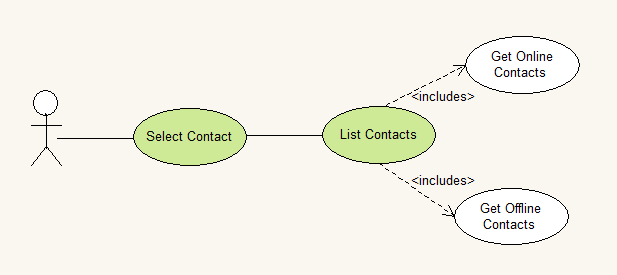
\includegraphics[width=6.0in, height=2.5in]{./viewContactsCase.png} \\
			\\\caption{[Figure 4]View Contact List Use Case}
		\end{figure*}\\
		
		\\ \noindent\textbf{4.2.1 Services Contract}\\
		To be added.\\
		
		\noindent\textbf{4.2.2 Functional Requirements}
			\begin{itemize}
				\item View a contact’s status.
				\item Click on contact to open a chat with the chosen contact.
				\item All contacts are shown, online and offline.
				\item Gets the previous messages from the database, they can also be viewed.\\
			\end{itemize}
\newpage
		\\ \left\textbf{4.2.3 Sequence Diagram} \\
			\begin{figure*}
				\centering
				 \\ 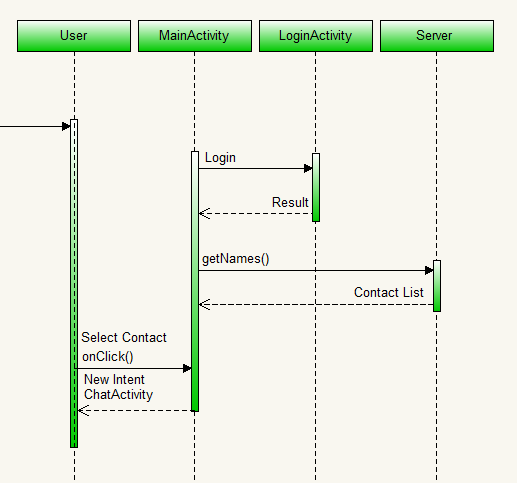
\includegraphics[width=5.5in, height=5.0in]{./viewContactsActivity.png}
				\\\caption{[Figure 5]View Contact List Activity Diagram}
			\end{figure*}	
\newpage
	\\ \left\textbf{4.3 Messaging Use Case} \\
		\begin{figure*}
			\centering
			\\ 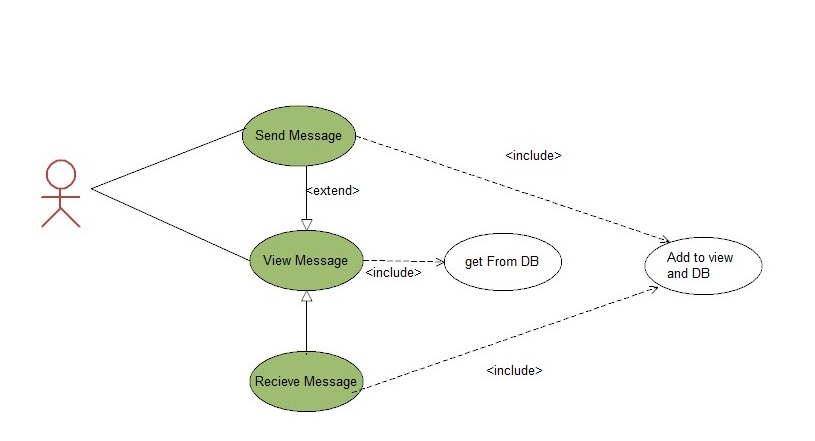
\includegraphics[width=6.0in, height=3.5in]{./messagingUseCase.jpg}
			\\\caption{[Figure 6]Messaging Use Case}\\
		\end{figure*}

		\noindent\textbf{4.3.1 Services Contract}\\
		To be added.\\
		
		\noindent\textbf{4.3.2 Functional Requirements}
			\begin{itemize}
				\item You can view previous messages.
				\item Send a new messages. New message is stored in the db.
				\item Offline and online messages are received instantly.
			\end{itemize}
			
\newpage
		\textbf{4.3.3 Sequence Diagram}
			\begin{figure*}
				\centering
				\\ 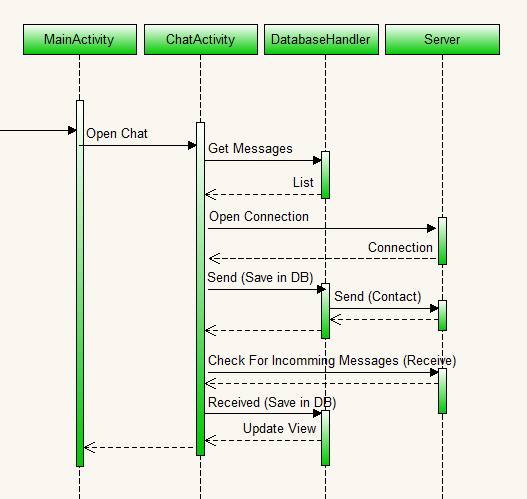
\includegraphics[width=5.5in, height=5.0in]{./mesActivity.png}
				\\\caption{[Figure 7]Messaging Activity Diagram}\\
			\end{figure*}	
		
\newpage		
	\left\textbf{4.4 Exit Use Case}
		\begin{figure*}
			\centering
			\\ 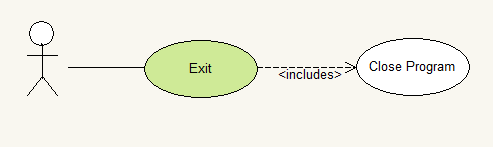
\includegraphics[width=6.0in, height=1.5in]{./exitCase.png}
			\\\caption{[Figure 8]Exit Use Case}\\
		\end{figure*}
		
		\noindent\textbf{4.4.1 Services Contract}\\ 
		To be added.\\
		\textbf{4.4.2 Functional Requirements}
			\begin{itemize}
				\item Ends the application on the device.\\
			\end{itemize}
		\left\textbf{4.4.3 Sequence Diagram}
		\begin{figure*}
			\centering
			\\ 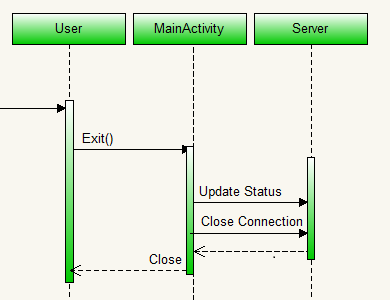
\includegraphics[width=4.0in, height=3.0in]{./exitActivity.png}
			\\\caption{[Figure 9]Exit Activity Diagram}
		\end{figure*}
		
\newpage		
	\left\textbf{4.5 MimeTeX Use Case}
		\begin{figure*}
			\centering
			\\ 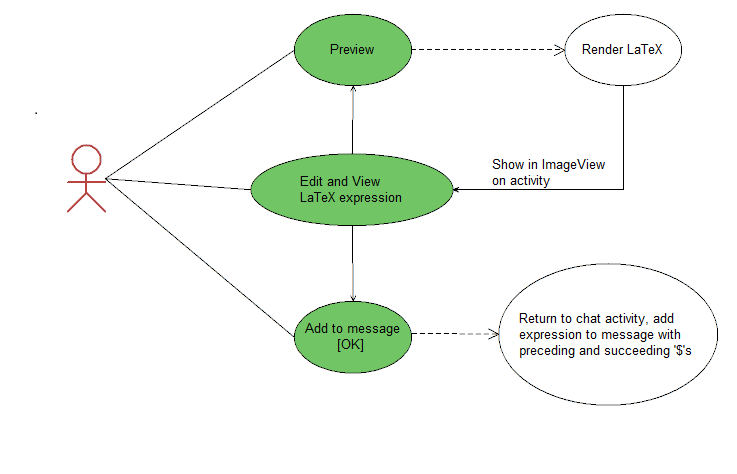
\includegraphics[width=6.0in, height=3.0in]{./MimeTeXUseCase.png}
			\\\caption{[Figure 10]MimeTeX Use Case}\\
		\end{figure*}
		
		\noindent\textbf{4.5.1 Services Contract}\\ 
		To be added.\\
		\textbf{4.5.2 Functional Requirements}
			\begin{itemize}
				\item Render LaTeX equations.\\
				\item Allows for preview of equations\\
			\end{itemize}
\newpage
		\left\textbf{4.5.3 Activity Diagram}
		\begin{figure*}
			\centering
			\\ 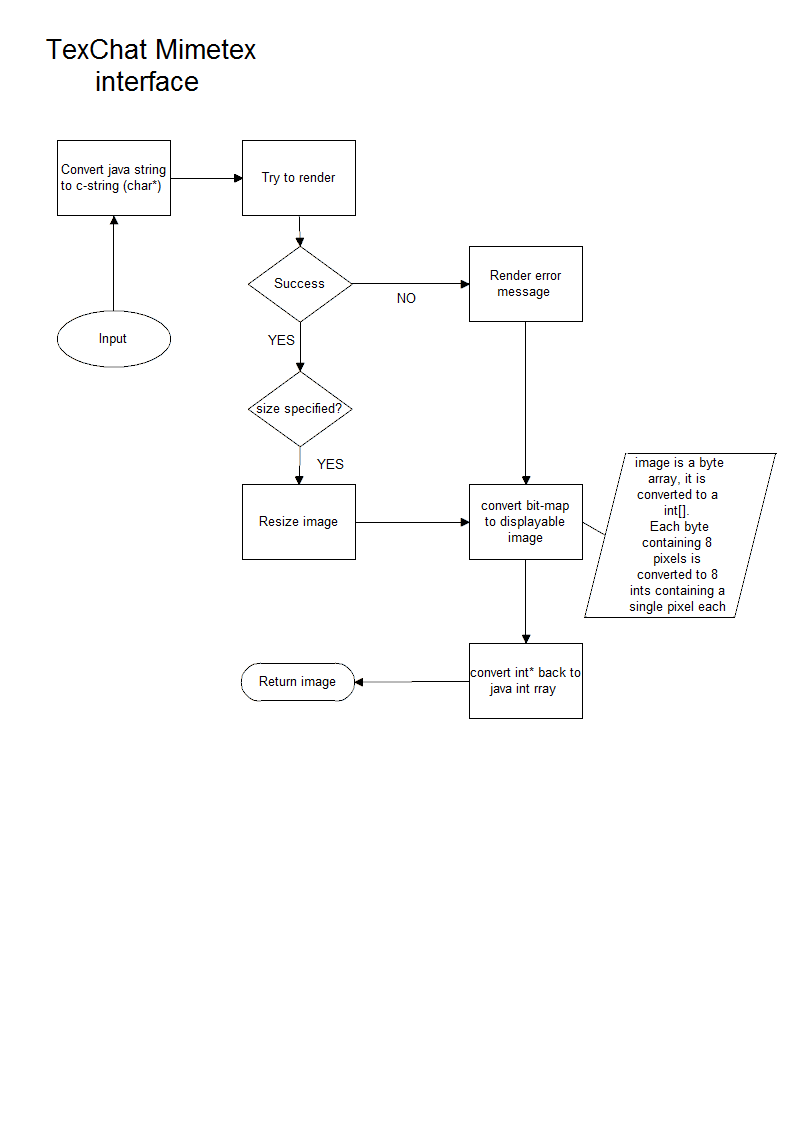
\includegraphics[width=6.0in, height=8.0in]{./activityMimeTex.png}
			\\\caption{[Figure 11]MimeTeX Activity Diagram}
		\end{figure*}
\newpage
	\section*{\textbf{5. Policies}}
	\vspace{4mm}
		\begin{itemize}
			\item Following Google’s coding standards for the different languages used.
			\item Using Google’s coding conventions.
			\item Software Development Methodology: Agile - RUP.
			\item Development will be mainly done using Java and XML and the Eclipse IDE, SDK, ADT and the NDK.
			\item The Android API will be used as a guideline and the API functions will be incorporated in the application.
			
		\end{itemize}	
	\vspace{5mm}
	
	\section*{\textbf{6. Open Issues}}
	\vspace{4mm}
		\begin{itemize}
			\item Styling
			\item Usability
			\item Testing and Integration Testing
			
		\end{itemize}
	\vspace{5mm}
	
	\section*{\textbf{7. Glossary}}
	\vspace{4mm}
		\begin{itemize}
			\item SDK - Software Development Kit
			\item NDK - Native Development Kit
			\item ADT - Android Development Toolkit plugin
			\item IDE - Integrated Development Environment
			\item RUP - Rational Unified Process
			\item XML - eXtensible Markup Language
			\item Agile - Development methodology
			\item MVC - Model View Controller
			\item UML - Unified Modelling Language
			\item API - Application Programming Interface
			\item MimeTex - LaTeX library ported to Android
			
		\end{itemize}
	\vspace{5mm}
\end{document}